\chapter{Wstęp}

Świat jest odwzorowywany przez programy komputerowe za pomocą modeli.
Zawierają one~uproszczoną reprezentację rzeczywistości, a logika programu
umożliwia wykonywanie obliczeń na podstawie modelu, jego modyfikację, lub
utrwalenie i udostępnienie do wglądu innym osobom.
Modele te mogą być prezentowane użytkownikowi na wiele sposobów. Jednym z~nich
jest reprezentacja graficzna w~formie diagramu. Taka metoda reprezentacji
pozwala użytkownikowi na łatwiejsze zrozumienie modelu
oraz jego modyfikację, w porównaniu do~formatu tekstowego, ponieważ jest
wizualna i przestrzenna, a więc jest naturalniejszą formą dla mózgu człowieka.

Przykładem modeli z reprezentacją graficzną, które są zrozumiałe zarówno dla
człowieka, jak i maszyny, oraz
przydają się podczas wytwarzania oprogramowania, są modele korzystające
z~\emphgls{UML}~\cite{wikipedia-uml}. Przedstawiają
one strukturę klas w programie oraz zależności między klasami. Na ich podstawie
czytelnik może wysokopoziomowo zapoznać się~ze strukturą programu, a
odpowiednie narzędzia pozwolą wygenerować kod klas w danym języku
programowania, który może służyć jako początek do późniejszego rozwoju
aplikacji. Przykładowy model \emphgls{UML} został przedstawiony na
rysunku~\ref{rys:przykladowy-model-uml}.

\begin{figure}[!ht]
	\centering
	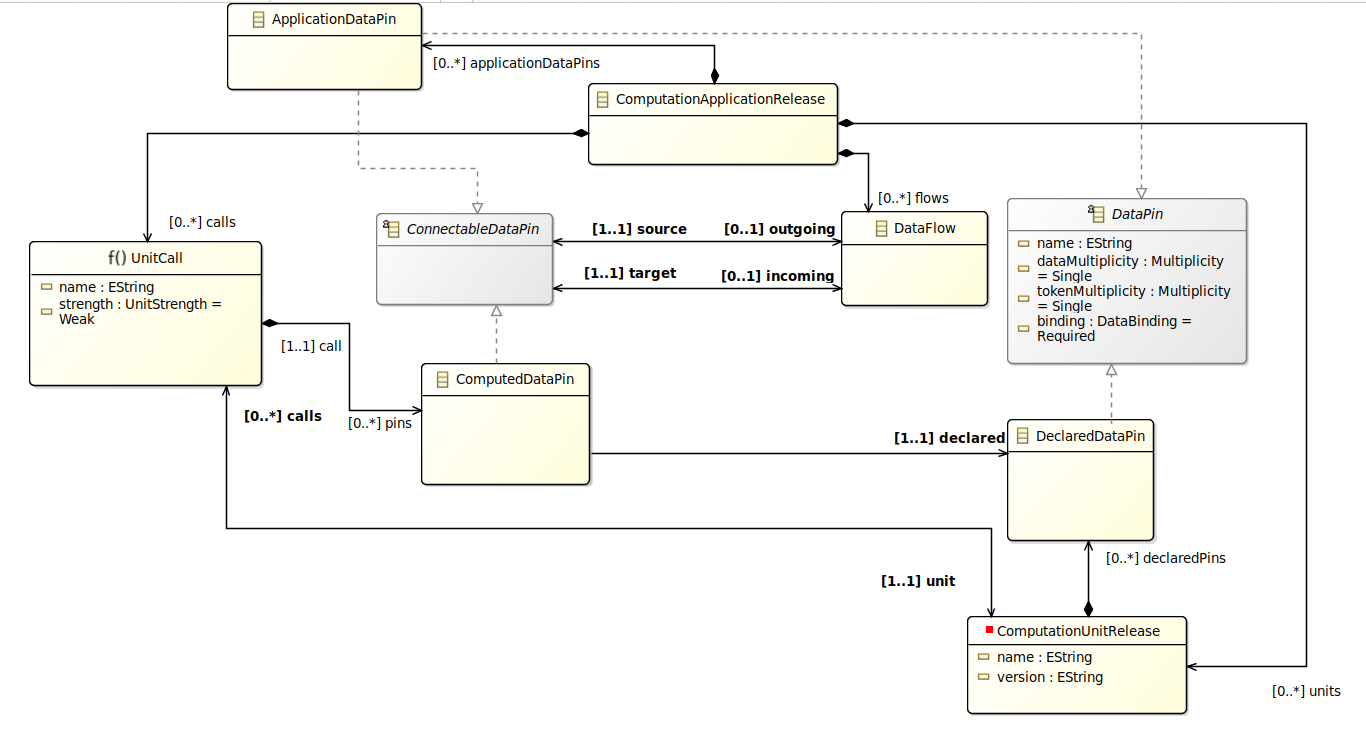
\includegraphics[width=0.95\linewidth]{./images/example-uml-model.png}
	\caption{Przykładowy model
		\emphgls{UML}}\label{rys:przykladowy-model-uml}
\end{figure}

\emphgls{UML} jest przykładem uniwersalnego języka do opisu modeli klas
programu.
Nie jest on~związany z żadną konkretną tematyką klas i pozwala na modelowanie
programów o~różnym zastosowaniu i przeznaczeniu. Istnieją także języki do opisu
modeli ściślej związanych z~konkretną dziedziną, czyli \emphgls{DSL}. Takie
języki
są zazwyczaj mniejsze i mniej skomplikowane od języków uniwersalnych, a także
mają dokładniejszą semantykę (znaczenie elementów modelu). Potrafią więc one
odwzorować rzeczywistość w~sposób bardziej kompletny i zawrzeć więcej
szczegółów.

Strukturę samego modelu opisuje metamodel. Jest to model, który definiuje jakie
są~możliwe typy elementów modelu, jakie mają atrybuty, jak są połączone ze
sobą (składnia języka modelowania). Sam metamodel może być opisany na przykład
w języku \emphgls{UML} lub podobnym
bazowanym na nim, który będzie umożliwiał wprowadzenie większej liczby
szczegółów. Taki metamodel często należy uzupełnić o zasady semantyczne ---
informacje o znaczeniu elementów, które nie mogą być zapisane w strukturze
metamodelu. Przykładową informacją semantyczną w modelu \emphgls{UML} może być
informacja o krotności asocjacji.

\BalticLSC{} jest platformą do obliczeń rozproszonych wykonywaną z
inicjatywy
\emph{INTERREG Regionu Morza Bałtyckiego Unit Europejskiej}. Platforma ta
pozwala
wykonać obliczenia wykorzystując dostępne moduły obliczeniowe. Aplikacje
obliczeniowe definiowane są w postaci diagramów przedstawiających przepływ
danych między modułami obliczeniowymi. Przykład diagramu opisującego aplikację
obliczeniową został przedstawiony na
rysunku~\ref{rys:przykladowy-diagram-balticlsc}.  Model obliczeń opisany jest w
języku \emphgls{CAL}, który jest opisany za pomocą
metamodelu~\cite{cal-metamodel}.

\begin{figure}[!ht]
	\centering

	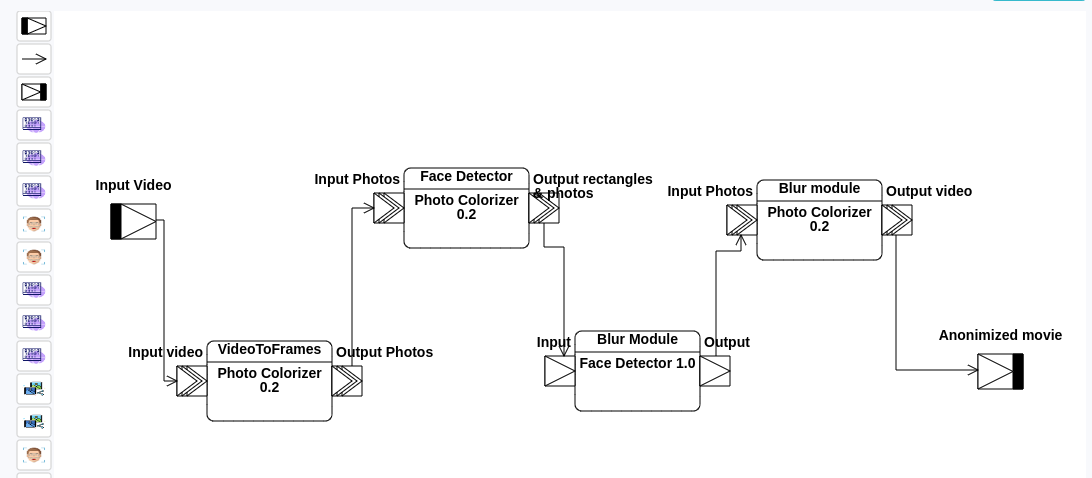
\includegraphics[width=0.95\linewidth]{./images/balticlsc-example-diagram.png}
	\caption{Przykładowy diagram przedstawiający aplikację obliczeniową w
		\BalticLSC{}}\label{rys:przykladowy-diagram-balticlsc}
\end{figure}

Istniejący edytor diagramów w \BalticLSC{} dostępny jest jako część aplikacji
przeglądarkowej udostępnionej przez platformę. Do komunikacji z aplikacją
serwerową wykorzystuje inną reprezentację aplikacji obliczeniowej --- zapisuje
ją w postaci pudełek (prostokątów) oraz połączeń między nimi. Nie komunikuje
się on z aplikacją serwerową przesyłając informacje o strukturze modelu
zgodnej z metamodelem języka \CAL{}. Sprawia to, że po obu stronach (serwera
i aplikacji przeglądarkowej) potrzebne są dodatkowe transformacje
przetwarzające ogólny opis diagramu na model aplikacji obliczeniowej.

\SiriusWeb{}~\cite{sirius-web-github} jest narzędziem przygotowywanym przez
firmę \emph{Eclipse} do tworzenia edytorów
diagramów działających w przeglądarce bazujących na metamodelach \EMF{}.
Technologia \EMF{} jest wykorzystywana od roku
2007~\cite{eclipse-sirius-wikipedia}, a metamodele
w~przeszłości mogły być tworzone używając oprogramowania \SiriusDesktop{}.
Wykorzystując \SiriusWeb{} można w prosty sposób otrzymać aplikację
przeglądarkową umożliwiającą możliwości przeglądania i edycji modeli zbliżone
do tych,
które dotychczas oferowała jedynie aplikacja wymagająca instalacji na
komputerze użytkownika. Oprócz łatwiejszego dostępu do edytora diagramów dla
nowych użytkowników, wykorzystanie technologii przeglądarkowych do budowy
edytora diagramów pozwala na dodanie mechanizmów kontroli dostępu do
wybranych modeli dla pewnych użytkowników, a także możliwości współpracy nad
modelem przez różne osoby w~czasie rzeczywistym.

W ustrukturyzowanym modelu zawierającym obiekty dziedzinowe w nietrudny sposób
można wyrazić reguły determinujące poprawność semantyczną modelu.
\SiriusDesktop{} pozwala w tym zakresie na definiowanie semantycznych reguł
walidacyjnych, które są uruchamiane po każdej modyfikacji modelu i pokazują
błędnie umieszczone elementy. Odpowiednik tej funkcjonalności jest pożądany
także w edytorach diagramów opartych na \SiriusWeb{}.

W ramach tej pracy magisterskiej przygotowany został edytor diagramów dla
systemu \BalticLSC{} korzystający z \SiriusWeb{}. Edytor ten bazuje na
formalnym metamodelu \EMF{} opisującym język \CAL{} do
opisu aplikacji obliczeniowej. Ponadto, dostarczona została metoda sprawdzania
poprawności przygotowywanych przez użytkownika modeli na podstawie
zdefiniowanych reguł walidacji.

\section{Motywacja i cel pracy}

Jedną z alternatyw do wykorzystania \SiriusWeb{} do budowy edytora diagramów
jest
wykorzystanie gotowych bibliotek \JavaScript{} do wyświetlania i modyfikacji
diagramów (przykłady: \emph{react-diagrams}~\cite{react-diagrams-github},
\emph{Cytoscape.js}~\cite{cytoscape-js-homepage},
\emph{vis-network}~\cite{vis-network-github}). Są one ogólnymi narzędziami
pozwalającymi na zbudowanie własnego edytora diagramów. Dają sporą dowolność w
kwestii wyświetlania diagramu oraz
dostępnych funkcjonalności. Nie narzucają one
wykorzystania ustrukturyzowanych modeli poprzez wymaganie stworzenia
metamodelu. Z uwagi na swoją ogólność są trudniejsze do dostosowania do
własnych potrzeb, ponieważ funkcjonalności takie jak zapisywanie modeli w bazie
danych, współpraca w czasie rzeczywistym, walidacja modelu należy
zaimplementować samemu. Ponadto, modyfikacja takiego edytora diagramów wymaga
znajomości języka \JavaScript{}.

\SiriusWeb{} dostarcza większość z tych
funkcjonalności wymagając jedynie wskazania metamodelu, który ma wykorzystywać.
Korzyści płynące z łatwego do przygotowania przeglądarkowego edytora diagramów
dla wybranych przez
nas modeli prezentują technologię \SiriusWeb{} jako interesującą i wartą
użycia,
pomimo jej wczesnej fazy rozwoju i braku dokumentacji.

Celem tej pracy magisterskiej jest zbadanie możliwości udostępnianych przez
\SiriusWeb{} poprzez wykorzystanie go do przygotowania edytora
diagramów dla modeli języka \CAL{}~na~platformie \BalticLSC{}. Elementem
edytora,
na który należy zwrócić szczególną uwagę, jest możliwość walidacji modeli,
czyli weryfikacji ich~poprawności strukturalnej i semantycznej.

Ponadto, praca ta będzie jednym z pierwszych zastosowań \SiriusWeb{} wykonanych
przez osoby spoza zespołu budującego tą technologię, co może dostarczyć
dodatkowych informacji zwrotnych na temat prostoty jego wykorzystania, a także
napotkanych błędów i~niedociągnięć. Dla osób rozważających budowę edytora
modeli w oparciu o \SiriusWeb{}, praca ta będzie stanowiła źródło informacji o
wrażeniach z wykorzystania tej technologii, co pomoże podjąć bardziej świadomą
decyzję o używanych technologiach.
Z uwagi na brak dostępnej dokumentacji \SiriusWeb{}, praca ta może służyć
również jako przykład wykorzystania własnego metamodelu w tym edytorze
diagramów.

Taki edytor diagramów bazujący na \SiriusWeb{} mógłby również zostać
wykorzystany
w~aplikacji przeglądarkowej platformy \BalticLSC{}. Jest on oparty o
ustrukturyzowany opis modelu, co pozwoliłoby na uproszczenie metody komunikacji
między serwerem aplikacyjnym a~aplikacją przeglądarkową, ponieważ nie byłyby
wymagane transformacje z aktualnego, ogólnego formatu danych do formatu
zgodnego z metamodelem.

\section{Zakres pracy}

W ramach pracy magisterskiej wykonano następujące czynności:

\begin{itemize}
	\item Stworzenie metamodelu języka \CAL{} w \EMF{}\@ z wykorzystaniem \SiriusDesktop{}.
	\item Wykorzystanie tego metamodelu w \SiriusWeb{}. Zgłoszenie usterek autorom \SiriusWeb{} poprzez \GitHub{}.
	\item Porównanie możliwości \SiriusWeb{} i \SiriusDesktop{}. Zgłoszenie brakujących funkcjonalności autorom \SiriusWeb{} poprzez \GitHub{}.
	\item Dodanie do metamodelu elementów usprawniających pracę z nim (automatyzacja niektórych czynności, dodanie ograniczeń utrudniających zrobienie błędu).
	\item Modyfikacja przeglądarkowego interfejsu użytkownika \SiriusWeb{} poprzez dodanie do~niego przybornika z \BalticLSC{}. Przybornik umożliwia w łatwy sposób dodanie nowych elementów do modelu.
	\item Dodanie mechanizmu walidacji semantycznej modelu sprawdzającego poprawność modelu z regułami zdefiniowanymi w języku \Java{}.
	\item Stworzenie planu integracji rozwiązania z \BalticLSC{}.
	\item Stworzenie przykładowej aplikacji przeglądarkowej zawierającej jedynie edytor diagramów z \SiriusWeb{}. Taki przykład pokazuje możliwość wykorzystania \SiriusWeb{} jako element innej aplikacji przeglądarkowej.
\end{itemize}

\vspace{1em}

\noindent Poza zakresem pracy pozostały następujące czynności:

\begin{itemize}
	\item Integracja stworzonego rozwiązania jako alternatywnego edytora diagramów dla systemu \BalticLSC{}.
	\item Naprawa zgłoszonych usterek w \SiriusWeb{}.
\end{itemize}
